\documentclass{standalone}
\usepackage{tikz}
\usepackage{verbatim}
\begin{document}
\pagestyle{empty}
  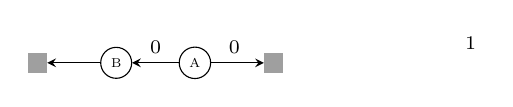
\begin{tikzpicture}
    \node[draw,rectangle,fill,gray!75] (l) at (-3, 0) {};
    \node[draw,circle,scale=2/3] (b) at (-2, 0) {\scriptsize B};
    \node[draw,circle,scale=2/3] (a) at (-1, 0) {\scriptsize A};
    \node[draw,rectangle,fill,gray!75] (r) at (0, 0) {};
    \draw[-stealth]  (b) -- (l);
    \draw[-stealth] (a) -- (b);
    \draw[-stealth]  (a) -- (r);
	 \node at (-1.5, 0.2) {\scriptsize 0};
	 \node at (-.5, 0.2) {\scriptsize 0};
    \node at (2.5, 0.25) {\scriptsize 1};
  \end{tikzpicture}
\end{document}